\documentclass[11pt]{standalone}
\usepackage{amssymb}
\usepackage{amsmath}
\usepackage[no-math]{fontspec}
\usepackage{unicode-math}
\setmainfont{Libertinus Sans}
\setsansfont{Libertinus Sans}
\setmathfont{Libertinus Math}
\usepackage{pgf,xcolor}
\usepackage{tikz}
\usetikzlibrary{arrows.meta, backgrounds, calc}
\usepackage{pgfplots}
\pgfplotsset{compat=newest}
\usepackage{pifont}

\definecolor{my_darkgray}{HTML}{484949}
\definecolor{my_lightgray}{HTML}{F3F4F4}
\definecolor{my_darkblue}{HTML}{005A94}
\definecolor{my_lightblue}{HTML}{CCDEE9}
\definecolor{my_yellow}{HTML}{FFEC7F}
\definecolor{my_red}{HTML}{E60000}
\definecolor{my_orange}{HTML}{E87846}

\begin{document}
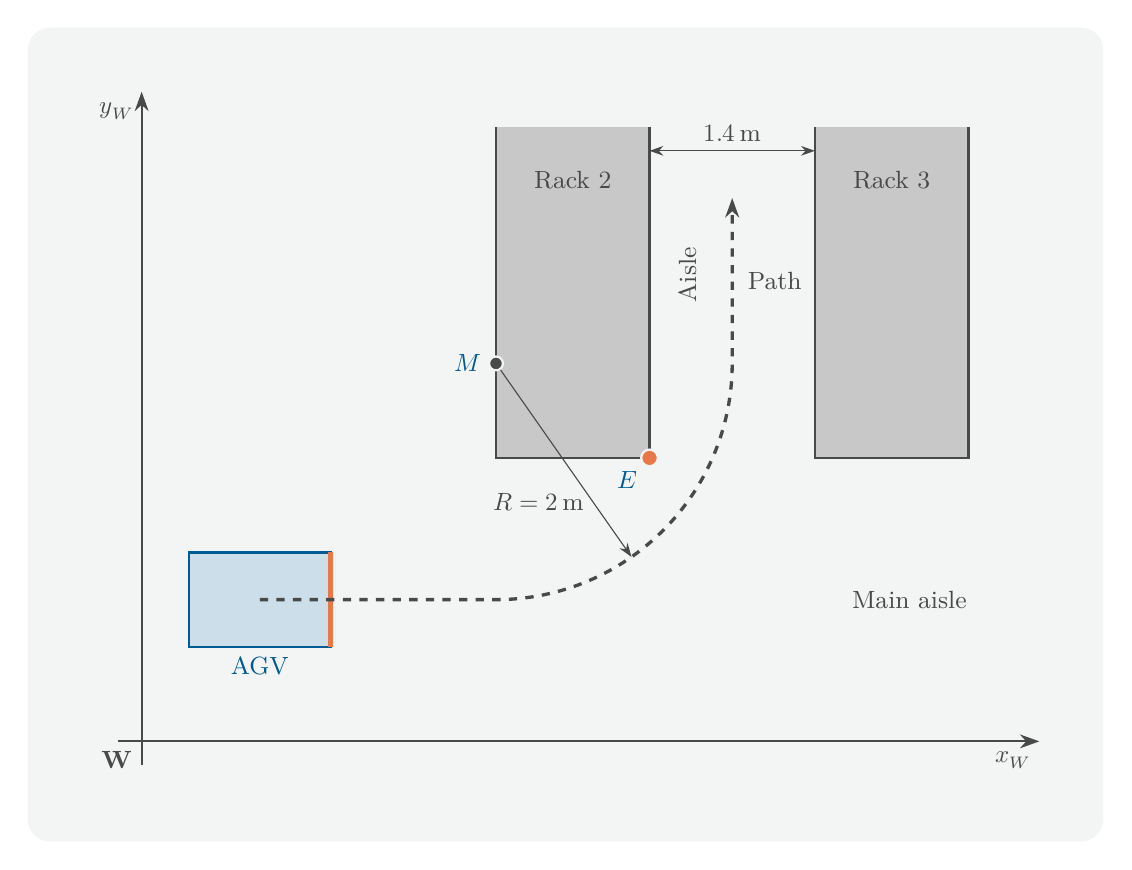
\begin{tikzpicture}[
    show background rectangle,
    background rectangle/.style={fill=my_lightgray, rounded corners=8pt},
    inner frame sep=0.8cm,
    x=1.5cm, y=1.5cm,
    achse/.style={thick, -{Stealth[length=7pt, width=5pt]}},
    bemassung/.style={draw=my_darkgray, thin, {Stealth[length=5pt, width=3.5pt]}-{Stealth[length=5pt, width=3.5pt]}},
    radiuspfeil/.style={draw=my_darkgray, thin, -{Stealth[length=5pt, width=3.5pt]}}
]

    % Draufsicht auf die Halle aus Kapitel 6.4, maßstäblich: 1 m = 1.5 cm.
    % Regale 2 und 3 ab y = 2.4 m, oben bei y = 5.2 m abgeschnitten (sie
    % reichen bis y = 7.5 m). Bahn: Gerade bei y = 1.2 m, Viertelkreis um
    % M = (3, 3.2) mit Radius 2 m, Gerade im Regalgang bei x = 5 m.
    \coordinate (M) at (3.0,3.2);
    \coordinate (E) at (4.3,2.4);

    % Weltkoordinatensystem W
    \draw[achse, draw=my_darkgray] (-0.2,0) -- (7.6,0)
        node[anchor=north east, font=\small, text=my_darkgray] {$x_W$};
    \draw[achse, draw=my_darkgray] (0,-0.2) -- (0,5.5)
        node[anchor=north east, font=\small, text=my_darkgray] {$y_W$};
    \node[font=\small\bfseries, text=my_darkgray, anchor=north east] at (0,0) {W};

    % Regale, nach oben offen gezeichnet
    \fill[my_darkgray!30] (3.0,2.4) rectangle (4.3,5.2);
    \draw[draw=my_darkgray, thick] (3.0,5.2) -- (3.0,2.4) -- (4.3,2.4) -- (4.3,5.2);
    \node[font=\small, text=my_darkgray] at (3.65,4.75) {Rack 2};
    \fill[my_darkgray!30] (5.7,2.4) rectangle (7.0,5.2);
    \draw[draw=my_darkgray, thick] (5.7,5.2) -- (5.7,2.4) -- (7.0,2.4) -- (7.0,5.2);
    \node[font=\small, text=my_darkgray] at (6.35,4.75) {Rack 3};

    % Beschriftung der Gänge
    \node[font=\small, text=my_darkgray, rotate=90] at (4.62,3.95) {Aisle};
    \node[font=\small, text=my_darkgray] at (6.5,1.2) {Main aisle};

    % Breite des Regalgangs
    \draw[bemassung] (4.3,5.0) -- (5.7,5.0)
        node[midway, anchor=south, font=\small, text=my_darkgray] {$1.4\,\text{m}$};

    % FTF am Start der Bahn: Umriss hellblau, Vorderkante orange
    \draw[fill=my_lightblue, draw=my_darkblue, thick] (0.4,0.8) rectangle (1.6,1.6);
    \draw[draw=my_orange, ultra thick] (1.6,0.8) -- (1.6,1.6);
    \node[font=\small, text=my_darkblue, anchor=north] at (1.0,0.8) {AGV};

    % Bahn: Gerade, Viertelkreis, Gerade
    \draw[draw=my_darkgray, very thick, dashed, -{Stealth[length=7pt, width=5pt]}]
        (1.0,1.2) -- (3.0,1.2) arc[start angle=-90, end angle=0, radius=2] -- (5.0,4.6);
    \node[font=\small, text=my_darkgray, anchor=west] at (5.05,3.9) {Path};

    % Mittelpunkt M und Radius R
    \draw[radiuspfeil] (M) -- ($(M)+(-55:2)$);
    \node[font=\small, text=my_darkgray, anchor=east] at ($(M)!0.72!($(M)+(-55:2)$)$)
        {$R = 2\,\text{m}$};
    \draw[fill=my_darkgray, draw=my_lightgray, thick] (M) circle (2.5pt);
    \node[font=\small, text=my_darkblue, anchor=east] at ($(M)+(-0.06,0)$) {$M$};

    % Regalecke E
    \draw[fill=my_orange, draw=my_lightgray, thick] (E) circle (3pt);
    \node[font=\small, text=my_darkblue, anchor=north east] at ($(E)+(-0.03,-0.03)$) {$E$};

\end{tikzpicture}
\end{document}
